\chapter{Edge disjoint path problem}

Some readers may already know what is edge disjoint path problem and also some basic algorithms. But we will have a brief introduction to this topic.

\begin{itemize}
	\item \textbf{INPUT}: $G=(V,E)$ and $(s_{i}, t_{i}) \in V^2$ for all $i \in [k]$.
	\item \textbf{OUTPUT}: $I \subseteq [k]$ and an $s_{i}-t_{i}$ path $P_{i}$ for each $i \in I$, s.t. the selected paths are edge disjoint.
	\item \textbf{OBJECTIVE}: $\max |I|$.
\end{itemize}

It is known that this particular problem is NP-hard. So we will again show some approximation to this problem. \textit{Note: for any fix $k$ it is solvable in polynomial time on undirected graph. But for directed graphs it is NP-hard for $k = 2$.} We will introduce an greedy algorithm that has an parameter.

\begin{algorithm}
	\caption{Greedy algorithm with a catch for parameter $\sqrt{m}$}
	\begin{algorithmic}[1]
		\State $I = \emptyset$
		\While{$\exists i \notin I$ and $\exists s_{i}-t_{i}$ path in $G$, s.t. $|P_{i}| \leq \sqrt{m}$}
			\State $I = I \cup \{i\}$, keep $P_{i}$, $G = G \setminus P_{i}$
		\EndWhile
	\end{algorithmic}
\end{algorithm}

We will denote $OPT$ as the optimal solution of the problem. It will be either a set of paths or set of indexes. Then we will denote $OPT_{S} = \{P \in OPT \mid |P| \leq \sqrt{m}\}$, where the length of a path is set as the number of edges. Then $OPT_{L} = OPT \setminus OPT_{S}$ and $ALG$ as the set given by the algorithm.

Now take the set $OPT_{S} \setminus ALG$. That is path between $s_{i}$ and $t_{i}$ is in this set if there exists $s_{j}-t_{j}$ path obtained by the algorithm which shares an edge. This path has length at most $\sqrt{m}$ and there are $|ALG|$ paths. Thus altogether $|OPT_{S} \setminus ALG| \leq \sqrt{m} |ALG|$.

Next we may see that $|OPT_{L}| \leq \sqrt{m}$, because we have $m$ edges and each one of them is at least $\sqrt{m}$ long. Now we may conclude altogether following result.

$$
|OPT| \leq |OPT_{L}| + |OPT_{S} \setminus ALG| + |ALG| \leq O(\sqrt{m}) |ALG|
$$

Now one can see where the catch in the algorithm is. Consider that there are no such short paths. The algorithm will output no path at all. To fix this we need to change the algorithm such that it will always output at least one path. If there is none then $OPT$ is 0 as well.

\begin{algorithm}
	\caption{Greedy ($\sqrt{m}$)}
	\begin{algorithmic}[1]
		\State $I = \emptyset$
		\While{$\exists i \notin I$ and $\exists s_{i}-t_{i}$ path in $G$, s.t. $|P_{i}| \leq \sqrt{m}$}
		\State $I = I \cup \{i\}$, keep $P_{i}$, $G = G \setminus P_{i}$
		\EndWhile
		\If{\textit{$I = \emptyset$}}
			\State \textit{Connect any $s_{i}-t_{i}$ path if possible.}
		\EndIf
	\end{algorithmic}
\end{algorithm}

Thus we have shown an algorithm that is a $\sqrt{m}$-approximation. Now we consider running the same algorithm but we change the parameter from $\sqrt{m}$ to $n^{2/3}$. Can we obtain $n^{2/3}$-approximation?

\begin{thm}[Khana, Chedari]
	\label{max flow bounded}
	Given an instance of the sum multi-commodity flow problem $G =(V,E)$, \newline $(s_{i}, t_{i}) \in V^2$ for all $i \in [k]$ such that $(\forall i) \ d(s_{i}, t_{i}) \geq l$, then the max multi-commodity flow is $O(\frac{n^2}{l^2})$.
\end{thm}

Before proving this we will show the consequences for our problem. Lets use the algorithm Greedy$(n^{2/3})$. Assume there $\exists P_{i} \in ALG, |P_{i}| \leq n^{2/3}$. Otherwise we use the theorem on the network obtained by $G$ and setting all capacities to one. Then all edges are at least $n^{2/3}$ length so we get the max multi-commodity flow is $O(\frac{n^{2}}{n^{4/3}}) = O(n^{2/3})$. Therefore it means if we choose just one path the approximation ratio will still be $O(n^{2/3})$.

Denote $OPT_{easy} = \{P \in OPT \mid \exists Q \in ALG : Q \cap P \neq \emptyset\}$. With this we know that $|OPT_{easy}| \leq n^{2/3} |ALG|$ by the same argument as it was already mentioned before.

We will look at $\forall (s_{i}, t_{i}) \in (OPT \setminus OPT_{easy}) \setminus ALG$. What can we say about such $d(s_{i}, t_{i})$ at the end of the loop of the algorithm. Clearly because it was not chosen either there is some intersection with another path, but this is remove by $OPT_{easy}$, so the other option is only that $d(s_{i}, t_{i}) > n^{2/3}$. Hence $|(OPT \setminus OPT_{easy}) \setminus ALG| \leq O(n^{2/3})$ by the theorem and the same argument which was already mentioned. Altogether we have:

$$
|OPT| \leq |OPT_{easy}| + |(OPT \setminus OPT_{easy}) \setminus ALG| + |ALG| = O(n^{2/3}) |ALG|
$$

Now we only need to prove the theorem since it is the base of our arguments for obtaining $O(n^{2/3})$-approximation algorithm.

\begin{proof}
	We will split the vertices into two sets:
	
	\begin{enumerate}
		\item \textbf{low degree vertex} is when $\deg(v) \leq \frac{6 n}{l}$
		\item \textbf{high degree vertex} is when $\deg(v) > \frac{6 n}{l}$
	\end{enumerate}
	
	Also we will assume $l$ is a multiple of 6. Otherwise it get lost in the $O$ notation. To finish the proof we will use an observation.
	
	\begin{observ}
		Any $s_{i}-t_{i}$ path (denote it as $s-t$) uses at least $l/6$ low degree vertices.
	\end{observ}
	
	\begin{proof}[Proof of observation]
		Consider running BFS on the graph starting from $s$. We denote $L_{i} = \{u \in V : d(s,u) = i\}$. Note that edges are only within one layer or only between adjacent layers. Let $B_{i}$ be a block of three consecutive layers $\{L_{3i}, L_{3i+1}, L_{3i+2}\}$. Because the length to $t$ is at least $l$ then there is at least $l/3$ blocks. Assume that $< l/6$ layers consists of only low degree vertices. Otherwise the observation obviously holds. Now discard all blocks containing a layer of only low degree vertices. As there are $\geq l/3$ blocks at least $\geq l/6$ blocks remain. Then the smallest remaining block is of size $\leq \frac{n}{l/6} = 6n/l$ which can be seen by pigeonhole principle. For the vertices in the middle layer we know all neighbors are within the block. Therefore it is a low degree vertex. This is a contradiction because we still have a block having one layer with low degree vertices only.
	\end{proof}
	
	Now for the theorem we know a \textbf{unit} of flow between any pair $s_{i}-t_{i}$ consumes $\mathbf{\Omega(l)}$ cpacity of edges adjacent to low degree vertices. And the total capacity adjacent to low degree vertices is $\leq n \deg(v) \leq n (6n/l) = O(n^2/l)$. Which gives us $O(n^2/l^2)$.
\end{proof}

This is an example of greedy algorithm and the fact that using it with different parameter may result in better approximation, but the analysis is way harder. We also saw using flows to limit paths, but this has also its limits. We will show a counterexample a graph called \textbf{Brick wall}.

\begin{figure}[!ht]\centering
	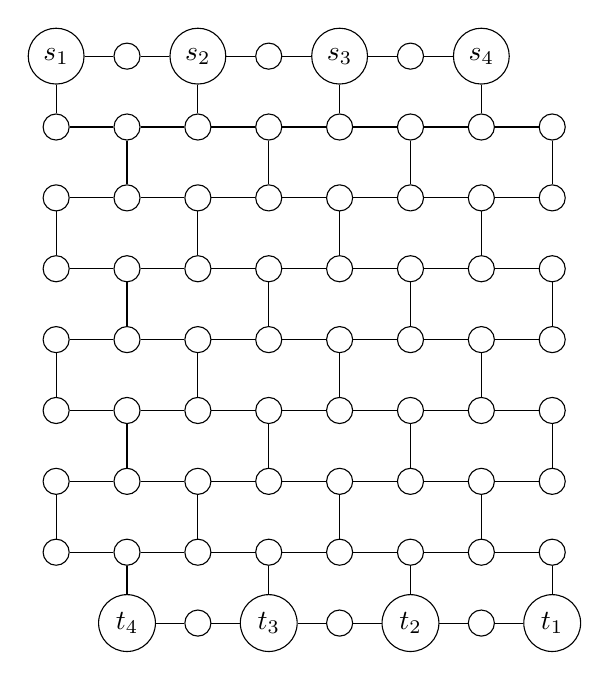
\begin{tikzpicture}[node distance={9mm}, main/.style = {draw, circle}]
		\node[main] (0) {$s_{1}$};
		\node[main] (1) [right of=0] {};
		\draw (0) -- (1);
		\node[main] (2) [right of=1] {$s_{2}$};
		\draw (1) -- (2);
		\node[main] (3) [right of=2] {};
		\draw (2) -- (3);
		\node[main] (4) [right of=3] {$s_{3}$};
		\draw (3) -- (4);
		\node[main] (5) [right of=4] {};
		\draw (4) -- (5);
		\node[main] (6) [right of=5] {$s_{4}$};
		\draw (5) -- (6);
		\node[main] (10) [below of=0] {};
		\draw (10) -- (0);
		\node[main] (11) [right of=10] {};
		\draw (11) -- (10);
		\node[main] (12) [right of=11] {};
		\draw (12) -- (11);
		\draw (12) -- (2);
		\node[main] (13) [right of=12] {};
		\draw (13) -- (12);
		\node[main] (14) [right of=13] {};
		\draw (14) -- (13);
		\draw (14) -- (4);
		\node[main] (15) [right of=14] {};
		\draw (15) -- (14);
		\node[main] (16) [right of=15] {};
		\draw (16) -- (15);
		\draw (16) -- (6);
		\node[main] (17) [right of=16] {};
		\draw (17) -- (16);
		\node[main] (20) [below of=10] {};
		\node[main] (21) [right of=20] {};
		\draw (21) -- (20);
		\draw (21) -- (11);
		\node[main] (22) [right of=21] {};
		\draw (22) -- (21);
		\node[main] (23) [right of=22] {};
		\draw (23) -- (22);
		\draw (23) -- (13);
		\node[main] (24) [right of=23] {};
		\draw (24) -- (23);
		\node[main] (25) [right of=24] {};
		\draw (25) -- (24);
		\draw (25) -- (15);
		\node[main] (26) [right of=25] {};
		\draw (26) -- (25);
		\node[main] (27) [right of=26] {};
		\draw (27) -- (26);
		\draw (27) -- (17);
		\node[main] (30) [below of=20] {};
		\draw (30) -- (20);
		\node[main] (31) [right of=30] {};
		\draw (31) -- (30);
		\node[main] (32) [right of=31] {};
		\draw (32) -- (31);
		\draw (32) -- (22);
		\node[main] (33) [right of=32] {};
		\draw (33) -- (32);
		\node[main] (34) [right of=33] {};
		\draw (34) -- (33);
		\draw (34) -- (24);
		\node[main] (35) [right of=34] {};
		\draw (35) -- (34);
		\node[main] (36) [right of=35] {};
		\draw (36) -- (35);
		\draw (36) -- (26);
		\node[main] (37) [right of=36] {};
		\draw (37) -- (36);
		\node[main] (40) [below of=30] {};
		\node[main] (41) [right of=40] {};
		\draw (41) -- (40);
		\draw (41) -- (31);
		\node[main] (42) [right of=41] {};
		\draw (42) -- (41);
		\node[main] (43) [right of=42] {};
		\draw (43) -- (42);
		\draw (43) -- (33);
		\node[main] (44) [right of=43] {};
		\draw (44) -- (43);
		\node[main] (45) [right of=44] {};
		\draw (45) -- (44);
		\draw (45) -- (35);
		\node[main] (46) [right of=45] {};
		\draw (46) -- (45);
		\node[main] (47) [right of=46] {};
		\draw (47) -- (46);
		\draw (47) -- (37);
		\node[main] (50) [below of=40] {};
		\draw (50) -- (40);
		\node[main] (51) [right of=50] {};
		\draw (51) -- (50);
		\node[main] (52) [right of=51] {};
		\draw (52) -- (51);
		\draw (52) -- (42);
		\node[main] (53) [right of=52] {};
		\draw (53) -- (52);
		\node[main] (54) [right of=53] {};
		\draw (54) -- (53);
		\draw (54) -- (44);
		\node[main] (55) [right of=54] {};
		\draw (55) -- (54);
		\node[main] (56) [right of=55] {};
		\draw (56) -- (55);
		\draw (56) -- (46);
		\node[main] (57) [right of=56] {};
		\draw (57) -- (56);
		\node[main] (60) [below of=50] {};
		\node[main] (61) [right of=60] {};
		\draw (61) -- (60);
		\draw (61) -- (51);
		\node[main] (62) [right of=61] {};
		\draw (62) -- (61);
		\node[main] (63) [right of=62] {};
		\draw (63) -- (62);
		\draw (63) -- (53);
		\node[main] (64) [right of=63] {};
		\draw (64) -- (63);
		\node[main] (65) [right of=64] {};
		\draw (65) -- (64);
		\draw (65) -- (55);
		\node[main] (66) [right of=65] {};
		\draw (66) -- (65);
		\node[main] (67) [right of=66] {};
		\draw (67) -- (66);
		\draw (67) -- (57);
		\node[main] (70) [below of=60] {};
		\draw (70) -- (60);
		\node[main] (71) [right of=70] {};
		\draw (71) -- (70);
		\node[main] (72) [right of=71] {};
		\draw (72) -- (71);
		\draw (72) -- (62);
		\node[main] (73) [right of=72] {};
		\draw (73) -- (72);
		\node[main] (74) [right of=73] {};
		\draw (74) -- (73);
		\draw (74) -- (64);
		\node[main] (75) [right of=74] {};
		\draw (75) -- (74);
		\node[main] (76) [right of=75] {};
		\draw (76) -- (75);
		\draw (76) -- (66);
		\node[main] (77) [right of=76] {};
		\draw (77) -- (76);
		\node[main] (81) [below of=71] {$t_{4}$};
		\node[main] (82) [right of=81] {};
		\draw (81) -- (71);
		\draw (82) -- (81);
		\node[main] (83) [right of=82] {$t_{3}$};
		\draw (83) -- (82);
		\node[main] (84) [right of=83] {};
		\draw (83) -- (73);
		\draw (84) -- (83);
		\node[main] (85) [right of=84] {$t_{2}$};
		\draw (85) -- (84);
		\node[main] (86) [right of=85] {};
		\draw (85) -- (75);
		\draw (86) -- (85);
		\node[main] (87) [right of=86] {$t_{1}$};
		\draw (77) -- (87);
		\draw (87) -- (86);
	\end{tikzpicture}
	\caption{Example of a \textbf{brick wall} graph for $k = 4$.}
	\label{brick-wall}
\end{figure}

The graph you may see at the picture \ref{brick-wall} is planar. Also it can be generalized to $k$ where there are $k$ pairs of bricks underneath. The edge disjoint problem optimum is 1, which we can see on picture \ref{edg}. And the max multi flow optimum is at least $k/2 = O(\sqrt{n})$, which can be seen on picture \ref{max-flow}.


\begin{figure}[!ht]\centering
	\begin{subfigure}{0.45\textwidth}\centering
		\begin{tikzpicture}[node distance={9mm}, main/.style = {draw, circle}]
			\node[main] (0) {$s_{1}$};
			\node[main] (1) [right of=0] {};
			\draw (0) -- (1);
			\node[main] (2) [right of=1] {$s_{2}$};
			\draw (1) -- (2);
			\node[main] (3) [right of=2] {};
			\draw (2) -- (3);
			\node[main] (4) [right of=3] {$s_{3}$};
			\draw (3) -- (4);
			\node[main] (5) [right of=4] {};
			\draw (4) -- (5);
			\node[main] (6) [right of=5] {$s_{4}$};
			\draw (5) -- (6);
			\node[main] (10) [below of=0] {};
			\draw (10) -- (0);
			\node[main] (11) [right of=10] {};
			\draw (11) -- (10);
			\node[main] (12) [right of=11] {};
			\draw (12) -- (11);
			\draw (12) -- (2);
			\node[main] (13) [right of=12] {};
			\draw (13) -- (12);
			\node[main] (14) [right of=13] {};
			\draw (14) -- (13);
			\draw (14) -- (4);
			\node[main] (15) [right of=14] {};
			\draw (15) -- (14);
			\node[main] (16) [right of=15] {};
			\draw (16) -- (15);
			\draw (16) -- (6);
			\node[main] (17) [right of=16] {};
			\draw (17) -- (16);
			\node[main] (20) [below of=10] {};
			\node[main] (21) [right of=20] {};
			\draw (21) -- (20);
			\draw (21) -- (11);
			\node[main] (22) [right of=21] {};
			\draw (22) -- (21);
			\node[main] (23) [right of=22] {};
			\draw (23) -- (22);
			\draw (23) -- (13);
			\node[main] (24) [right of=23] {};
			\draw (24) -- (23);
			\node[main] (25) [right of=24] {};
			\draw (25) -- (24);
			\draw (25) -- (15);
			\node[main] (26) [right of=25] {};
			\draw (26) -- (25);
			\node[main] (27) [right of=26] {};
			\draw (27) -- (26);
			\draw (27) -- (17);
			\node[main] (30) [below of=20] {};
			\draw (30) -- (20);
			\node[main] (31) [right of=30] {};
			\draw (31) -- (30);
			\node[main] (32) [right of=31] {};
			\draw (32) -- (31);
			\draw (32) -- (22);
			\node[main] (33) [right of=32] {};
			\draw (33) -- (32);
			\node[main] (34) [right of=33] {};
			\draw (34) -- (33);
			\draw (34) -- (24);
			\node[main] (35) [right of=34] {};
			\draw (35) -- (34);
			\node[main] (36) [right of=35] {};
			\draw (36) -- (35);
			\draw (36) -- (26);
			\node[main] (37) [right of=36] {};
			\draw (37) -- (36);
			\node[main] (40) [below of=30] {};
			\node[main] (41) [right of=40] {};
			\draw (41) -- (40);
			\draw (41) -- (31);
			\node[main] (42) [right of=41] {};
			\draw (42) -- (41);
			\node[main] (43) [right of=42] {};
			\draw (43) -- (42);
			\draw (43) -- (33);
			\node[main] (44) [right of=43] {};
			\draw (44) -- (43);
			\node[main] (45) [right of=44] {};
			\draw (45) -- (44);
			\draw (45) -- (35);
			\node[main] (46) [right of=45] {};
			\draw (46) -- (45);
			\node[main] (47) [right of=46] {};
			\draw (47) -- (46);
			\draw (47) -- (37);
			\node[main] (50) [below of=40] {};
			\draw (50) -- (40);
			\node[main] (51) [right of=50] {};
			\draw (51) -- (50);
			\node[main] (52) [right of=51] {};
			\draw (52) -- (51);
			\draw (52) -- (42);
			\node[main] (53) [right of=52] {};
			\draw (53) -- (52);
			\node[main] (54) [right of=53] {};
			\draw (54) -- (53);
			\draw (54) -- (44);
			\node[main] (55) [right of=54] {};
			\draw (55) -- (54);
			\node[main] (56) [right of=55] {};
			\draw (56) -- (55);
			\draw (56) -- (46);
			\node[main] (57) [right of=56] {};
			\draw (57) -- (56);
			\node[main] (60) [below of=50] {};
			\node[main] (61) [right of=60] {};
			\draw (61) -- (60);
			\draw (61) -- (51);
			\node[main] (62) [right of=61] {};
			\draw (62) -- (61);
			\node[main] (63) [right of=62] {};
			\draw (63) -- (62);
			\draw (63) -- (53);
			\node[main] (64) [right of=63] {};
			\draw (64) -- (63);
			\node[main] (65) [right of=64] {};
			\draw (65) -- (64);
			\draw (65) -- (55);
			\node[main] (66) [right of=65] {};
			\draw (66) -- (65);
			\node[main] (67) [right of=66] {};
			\draw (67) -- (66);
			\draw (67) -- (57);
			\node[main] (70) [below of=60] {};
			\draw (70) -- (60);
			\node[main] (71) [right of=70] {};
			\draw (71) -- (70);
			\node[main] (72) [right of=71] {};
			\draw (72) -- (71);
			\draw (72) -- (62);
			\node[main] (73) [right of=72] {};
			\draw (73) -- (72);
			\node[main] (74) [right of=73] {};
			\draw (74) -- (73);
			\draw (74) -- (64);
			\node[main] (75) [right of=74] {};
			\draw (75) -- (74);
			\node[main] (76) [right of=75] {};
			\draw (76) -- (75);
			\draw (76) -- (66);
			\node[main] (77) [right of=76] {};
			\draw (77) -- (76);
			\node[main] (81) [below of=71] {$t_{4}$};
			\node[main] (82) [right of=81] {};
			\draw (81) -- (71);
			\draw (82) -- (81);
			\node[main] (83) [right of=82] {$t_{3}$};
			\draw (77) -- (87);
			\draw (83) -- (82);
			\node[main] (84) [right of=83] {};
			\draw (83) -- (73);
			\draw (84) -- (83);
			\node[main] (85) [right of=84] {$t_{2}$};
			\draw (77) -- (87);
			\draw (85) -- (84);
			\node[main] (86) [right of=85] {};
			\draw (85) -- (75);
			\draw (86) -- (85);
			\node[main] (87) [right of=86] {$t_{1}$};
			\draw (77) -- (87);
			\draw (87) -- (86);
			\path[color=myblue, line width = 4] (0) edge (10)
			(10) edge (11)
			(11) edge (21)
			(21) edge (22)
			(22) edge (32)
			(32) edge (33)
			(33) edge (43)
			(43) edge (44)
			(44) edge (54)
			(54) edge (55)
			(55) edge (65)
			(65) edge (66)
			(66) edge (76)
			(76) edge (77)
			(77) edge (87);
		\end{tikzpicture}
		\caption{Edge disjoint problem.}
		\label{edg}
	\end{subfigure}\centering
	\begin{subfigure}{0.45\textwidth}\centering
		\begin{tikzpicture}[node distance={9mm}, main/.style = {draw, circle}]
			\node[main] (0) {$s_{1}$};
			\node[main] (1) [right of=0] {};
			\draw (0) -- (1);
			\node[main] (2) [right of=1] {$s_{2}$};
			\draw (1) -- (2);
			\node[main] (3) [right of=2] {};
			\draw (2) -- (3);
			\node[main] (4) [right of=3] {$s_{3}$};
			\draw (3) -- (4);
			\node[main] (5) [right of=4] {};
			\draw (4) -- (5);
			\node[main] (6) [right of=5] {$s_{4}$};
			\draw (5) -- (6);
			\node[main] (10) [below of=0] {};
			\draw (10) -- (0);
			\node[main] (11) [right of=10] {};
			\draw (11) -- (10);
			\node[main] (12) [right of=11] {};
			\draw (12) -- (11);
			\draw (12) -- (2);
			\node[main] (13) [right of=12] {};
			\draw (13) -- (12);
			\node[main] (14) [right of=13] {};
			\draw (14) -- (13);
			\draw (14) -- (4);
			\node[main] (15) [right of=14] {};
			\draw (15) -- (14);
			\node[main] (16) [right of=15] {};
			\draw (16) -- (15);
			\draw (16) -- (6);
			\node[main] (17) [right of=16] {};
			\draw (17) -- (16);
			\node[main] (20) [below of=10] {};
			\node[main] (21) [right of=20] {};
			\draw (21) -- (20);
			\draw (21) -- (11);
			\node[main] (22) [right of=21] {};
			\draw (22) -- (21);
			\node[main] (23) [right of=22] {};
			\draw (23) -- (22);
			\draw (23) -- (13);
			\node[main] (24) [right of=23] {};
			\draw (24) -- (23);
			\node[main] (25) [right of=24] {};
			\draw (25) -- (24);
			\draw (25) -- (15);
			\node[main] (26) [right of=25] {};
			\draw (26) -- (25);
			\node[main] (27) [right of=26] {};
			\draw (27) -- (26);
			\draw (27) -- (17);
			\node[main] (30) [below of=20] {};
			\draw (30) -- (20);
			\node[main] (31) [right of=30] {};
			\draw (31) -- (30);
			\node[main] (32) [right of=31] {};
			\draw (32) -- (31);
			\draw (32) -- (22);
			\node[main] (33) [right of=32] {};
			\draw (33) -- (32);
			\node[main] (34) [right of=33] {};
			\draw (34) -- (33);
			\draw (34) -- (24);
			\node[main] (35) [right of=34] {};
			\draw (35) -- (34);
			\node[main] (36) [right of=35] {};
			\draw (36) -- (35);
			\draw (36) -- (26);
			\node[main] (37) [right of=36] {};
			\draw (37) -- (36);
			\node[main] (40) [below of=30] {};
			\node[main] (41) [right of=40] {};
			\draw (41) -- (40);
			\draw (41) -- (31);
			\node[main] (42) [right of=41] {};
			\draw (42) -- (41);
			\node[main] (43) [right of=42] {};
			\draw (43) -- (42);
			\draw (43) -- (33);
			\node[main] (44) [right of=43] {};
			\draw (44) -- (43);
			\node[main] (45) [right of=44] {};
			\draw (45) -- (44);
			\draw (45) -- (35);
			\node[main] (46) [right of=45] {};
			\draw (46) -- (45);
			\node[main] (47) [right of=46] {};
			\draw (47) -- (46);
			\draw (47) -- (37);
			\node[main] (50) [below of=40] {};
			\draw (50) -- (40);
			\node[main] (51) [right of=50] {};
			\draw (51) -- (50);
			\node[main] (52) [right of=51] {};
			\draw (52) -- (51);
			\draw (52) -- (42);
			\node[main] (53) [right of=52] {};
			\draw (53) -- (52);
			\node[main] (54) [right of=53] {};
			\draw (54) -- (53);
			\draw (54) -- (44);
			\node[main] (55) [right of=54] {};
			\draw (55) -- (54);
			\node[main] (56) [right of=55] {};
			\draw (56) -- (55);
			\draw (56) -- (46);
			\node[main] (57) [right of=56] {};
			\draw (57) -- (56);
			\node[main] (60) [below of=50] {};
			\node[main] (61) [right of=60] {};
			\draw (61) -- (60);
			\draw (61) -- (51);
			\node[main] (62) [right of=61] {};
			\draw (62) -- (61);
			\node[main] (63) [right of=62] {};
			\draw (63) -- (62);
			\draw (63) -- (53);
			\node[main] (64) [right of=63] {};
			\draw (64) -- (63);
			\node[main] (65) [right of=64] {};
			\draw (65) -- (64);
			\draw (65) -- (55);
			\node[main] (66) [right of=65] {};
			\draw (66) -- (65);
			\node[main] (67) [right of=66] {};
			\draw (67) -- (66);
			\draw (67) -- (57);
			\node[main] (70) [below of=60] {};
			\draw (70) -- (60);
			\node[main] (71) [right of=70] {};
			\draw (71) -- (70);
			\node[main] (72) [right of=71] {};
			\draw (72) -- (71);
			\draw (72) -- (62);
			\node[main] (73) [right of=72] {};
			\draw (73) -- (72);
			\node[main] (74) [right of=73] {};
			\draw (74) -- (73);
			\draw (74) -- (64);
			\node[main] (75) [right of=74] {};
			\draw (75) -- (74);
			\node[main] (76) [right of=75] {};
			\draw (76) -- (75);
			\draw (76) -- (66);
			\node[main] (77) [right of=76] {};
			\draw (77) -- (76);
			\node[main] (81) [below of=71] {$t_{4}$};
			\node[main] (82) [right of=81] {};
			\draw (81) -- (71);
			\draw (82) -- (81);
			\node[main] (83) [right of=82] {$t_{3}$};
			\draw (77) -- (87);
			\draw (83) -- (82);
			\node[main] (84) [right of=83] {};
			\draw (83) -- (73);
			\draw (84) -- (83);
			\node[main] (85) [right of=84] {$t_{2}$};
			\draw (77) -- (87);
			\draw (85) -- (84);
			\node[main] (86) [right of=85] {};
			\draw (85) -- (75);
			\draw (86) -- (85);
			\node[main] (87) [right of=86] {$t_{1}$};
			\draw (77) -- (87);
			\draw (87) -- (86);
			\path[color=myorange, line width = 4] (0) edge (10)
			(10) edge (11)
			(11) edge (21)
			(21) edge (22)
			(22) edge (32)
			(32) edge (33)
			(33) edge (43)
			(43) edge (44)
			(44) edge (54)
			(54) edge (55)
			(55) edge (65)
			(65) edge (66)
			(66) edge (76)
			(76) edge (77)
			(77) edge (87);
			\path[color=myviolet, line width = 4] (2) edge (12)
			(12) edge (13)
			(13) edge (23)
			(23) edge (24)
			(24) edge (34)
			(34) edge (35)
			(35) edge (45)
			(45) edge (46)
			(46) edge (56)
			(56) edge (57)
			(57) edge (67)
			(67) edge (66)
			(66) edge (65)
			(65) edge (64)
			(64) edge (74)	(74) edge (75)	(75) edge (85);
			\path[color=myblue, line width = 4] (4) edge (14)
			(14) edge (15)
			(15) edge (25)
			(25) edge (26)
			(26) edge (36)
			(36) edge (37)
			(37) edge (47)
			(47) edge (46)
			(46) edge (45)
			(45) edge (44)
			(44) edge (43)
			(43) edge (42)
			(42) edge (52)
			(52) edge (53)	(53) edge (63)	(63) edge (62)	(62) edge (72)	(72) edge (73)	(73) edge (83);
			\path[color=mygreen, line width = 4] (6) edge (16)
			(16) edge (17)
			(17) edge (27)
			(27) edge (26)
			(26) edge (25)
			(25) edge (24)
			(24) edge (23)
			(23) edge (22)
			(22) edge (21)
			(21) edge (20)
			(20) edge (30)
			(30) edge (31)	(31) edge (41)	(41) edge (40)	(40) edge (50)
			(50) edge (51)	(51) edge (61)	(61) edge (60)	(60) edge (70)	(70) edge (71)	(71) edge (81);
		\end{tikzpicture}
		\caption{Max multi flow; paths have $1/2$.}
		\label{max-flow}
	\end{subfigure}
	\caption{Example of optimalization problems.}
\end{figure}

\section{Edge disjoint path problem and flow number}

We will be again considering undirected graph $G=(V,E)$. And also a concurrent multi-commodity flow problem (or CMFP for short) with $(s_{i}, t_{i})$ commodities for $i = 1, \dots, k$ and their demands $d_{i} \in \R^{+}$. We will denote $S$ as a feasible solution for such problem.

\begin{defn}
	\textbf{Flow value} is the value of the objective function for $S$.
\end{defn}

\begin{defn}
	\textbf{Balanced instance} of the CMFP such that
	
	$$
	\forall v \in V(G) : \sum_{i: s_{i} = v} d_{i} = \deg(v) = \sum_{i: t_{i} = v} d_{i}.
	$$
\end{defn}

It may also be defined with inequalities. We will be calling this \textbf{balanced multi-commodity flow problem} (or BMFP for short).

\begin{defn}
	\textbf{Product multi-commodity flow} (PMFP for short) is an instance where
	
	\begin{itemize}
		\item There is a value $\pi(v) \in \R^+$ associated with every vertex $v \in V$.
		\item There is a commodity for every ordered pair of vertices $(u,v)$ of demand $\pi(u) \cdot \pi(v)$.
	\end{itemize}
\end{defn}

\begin{defn}
	\textbf{Dilation}$(S)$ denoted as $D(S)$ is the length of the longest path in $S$.
\end{defn}

\begin{defn}
	\textbf{Congestion}$(S)$ denoted as $C(S)$ is the inverse of the flow value in $S$.
\end{defn}

As a side-note when there was a problem for a networks in a computers to find best paths for sending packets it can be shown that the upper bound for the time is somewhat connected to similiar terms, particularly $O(C + D)$.

Now for a given $G = (V,E)$ we denote $I_{0}$ as an instance of the PMFP with $\pi(u) = \frac{\deg(u)}{\sqrt{2|E|}}$. \textit{Note that $2|E| = \sum_{v \in V} \deg(v)$.}

\begin{defn}
	\textbf{Flow number} of a graph $G$ denoted as $F(G)$ is
	
	$$
	\min_{\text{feasible solution } S \text{ for } I_{0}} \{ \max \{ C(S), D(S) \} \}
	$$
\end{defn}

\begin{claim}
	There is a polynomial time algorithm that computes $F(G)$ for every graph $G$.
\end{claim}

\begin{proof}
	Lets assume $V = \{v_{1}, v_{2}, \dots, v_{n}\}$. For $L \in \N$ we define graph $G_{L} = (V', E')$. This is a layered graph with $L+1$ layers. To be precise it is defined as follows
	
	$$
	\begin{aligned}
		V_{i} &= \{v_{i1}, v_{i2}, \dots, v_{in}\}, &\quad \forall i \in 0, 1, \dots, L \\
		E_{i} &= \{(v_{(i-1)j}, v_{ik}) \mid \{v_{j}, v_{k}\} \in E \} \cup \{(v_{(i-1)j}, v_{ij}) \mid v_{j} \in V\}, &\quad \forall i \in 1,2, \dots, L \\
	\end{aligned}
	$$
	
	$$
	\text{then } V' = \bigcup_{i = 0}^{L} V_{i} \text{ and } E' = \bigcup_{i=1}^{L} E_{i}.
	$$
	
	Note that we do not keep $V$ and $E$ from the original graph.
	
	Now consider the following instance of CMFP. $\forall (v_{i}, v_{j}) \in V^2$ we set commodity between $v_{0i}$ and $v_{Lj}$ of demand $\pi(v_{i}) \cdot \pi(v_{j})$ (where $\pi$ is taken from $I_{0}$). We also define a special request. $\forall \{v_{i}, v_{j}\} \in E$ the sum of flows over all edges in
	
	$$
	\bigcup_{k = 1}^{L} \{ (v_{(k-1)i}, v_{kj}), (v_{(k-1)j}, v_{ki}) \}
	$$
	
	has to be at most 1. This is just a linear constrained so we are able to solve this in polynomial time. With this requirement we are able to map the solution to the original graph $G$. Also the dilation is $L$ and to compute the congestion is easy to do from the result of LP. In other words $\forall L \in \{1, \dots, |V|\}$ find opt of this LP in $G_{L}$ and denote it as $S_{L}$. Then let $S_{L}'$ be the corresponding flow in $G$. Hence the following holds.
	
	$$
	F(G) = \min_{L = 1, \dots, |V|} \{ \max \{ C(S_{L}'), D(S_{L}')\} \}
	$$
\end{proof}

\begin{figure}[!ht]\centering
	\begin{subfigure}{0.45\textwidth}\centering
		\begin{tikzpicture}[node distance={13mm}, main/.style = {draw, thick, circle}]
			\node[main] (a) [] {$a$};
			\node[main] (b) [below of=a] {$b$};
			\node[main] (c) [right of=a] {$c$};
			\node[main] (d) [right of=b] {$d$};
			\draw[color=myblue, thick] (a) edge (d);
			\draw[color=myred, thick] (b) edge (d);
			\draw[color=myviolet, thick] (c) edge (d);
		\end{tikzpicture}
		\caption{Original graph $G$.}
	\end{subfigure}
	\begin{subfigure}{0.45\textwidth}\centering
		\begin{tikzpicture}[node distance={20mm}, main/.style = {draw, thick, circle}]
			\node[main] (a1) [] {$a_{1}$};
			\node[main] (b1) [right of=a1] {$b_{1}$};
			\node[main] (c1) [right of=b1] {$c_{1}$};
			\node[main] (d1) [right of=c1] {$d_{1}$};
			
			\node[main] (a2) [below of=a1] {$a_{2}$};
			\node[main] (b2) [right of=a2] {$b_{2}$};
			\node[main] (c2) [right of=b2] {$c_{2}$};
			\node[main] (d2) [right of=c2] {$d_{2}$};
			
			\node[main] (a3) [below of=a2] {$a_{3}$};
			\node[main] (b3) [right of=a3] {$b_{3}$};
			\node[main] (c3) [right of=b3] {$c_{3}$};
			\node[main] (d3) [right of=c3] {$d_{3}$};
			
			\path[->, thick] (a1) edge (a2) (a2) edge (a3);
			\path[->, thick] (b1) edge (b2) (b2) edge (b3);
			\path[->, thick] (c1) edge (c2) (c2) edge (c3);
			\path[->, thick] (d1) edge (d2) (d2) edge (d3);
			
			\path[->, color=myblue, thick] (a1) edge (d2) (d1) edge (a2)
			                             (a2) edge (d3) (d2) edge (a3);
			                               
			\path[->, color=myred, thick] (b1) edge (d2) (d1) edge (b2)
			                            (b2) edge (d3) (d2) edge (b3);
			
			\path[->, color=myviolet, thick] (c1) edge (d2) (d1) edge (c2)
			                               (c2) edge (d3) (d2) edge (c3);
			
		\end{tikzpicture}
		\caption{Layered graph $G_{L}$ for $L = 3$.}
	\end{subfigure}
	\caption{Shown a visualization of a graph $G$ and its layered version $G_{L}$.}
\end{figure}

\begin{claim}
	For any graph $G$ with flow number $F = F(G)$ and an instance $I$ of the BMFP in $G$, there is a feasible solution for $I$ with congestion and dilation at most $2F$.
\end{claim}

\begin{proof}
	For every $(s_{i}, t_{i}) \in I$ we define two instances:
	
	$$
	\begin{aligned}
		I_{1} &: \forall u \in V \text{ add commodity } (s_{i}, u) \text{ of demand } \frac{d_{i} \deg(u)}{2|E|} \\
		I_{2} &: \forall u \in V \text{ add commodity } (u, t_{i}) \text{ of demand } \frac{d_{i} \deg(u)}{2|E|} \\
	\end{aligned}
	$$
	
	Note that $\sum_{v \in V} \frac{d_{i} \deg(v)}{2|E|} = d_{i}$. For $v,w$ what is the sum of demands between $v$ and $w$ in $I_{1}$?
	
	$$
	\sum_{i: s_{i} = v} \frac{d_{i} \deg(w)}{2|E|} = \frac{\deg(w)}{2|E|} \sum_{i: s_{i} = v} d_{i} = \frac{\deg(w)}{2|E|} \deg(v) = \frac{\deg(w) \deg(v)}{2|E|}
	$$
	
	This means that $I_{1}$ is actually $I_{0}$. Similarly it can be shown that $I_{2} = I_{0}$. Hence the $F$ will be doubled for both $I_{1}$ and $I_{2}$ thus getting at most $2F$.
\end{proof}

\begin{lemma}[Flow shortening]
	Let $G = (V,E)$ be a graph and $F = F(G)$ be its flow number. For any $\epsilon \in [0,1]$ and any feasible flow $S$ in $G$ of flow value $f$, for an instance of CMFP. There exists a feasible flow of flow value $\geq \frac{f}{1+\epsilon}$ that uses paths of lengths $\leq 2F(1+\frac{1}{\epsilon})$.
\end{lemma}

Before we properly show the proof we show the idea behind it. We set $L = \frac{2F}{\epsilon}$ and for every path we find the first $L$ vertices and last $L$ vertices. In some paths they may overlap. We will connect the opposite vertices and scale demands and flows, so it will eventually work.

\begin{proof}
	Denote $\mathcal{O}$ the set of the paths in $S$. For $p \in \mathcal{O}$ denote $f_{p}$ as the amount of flow on path $p$. Now let $\mathcal{O}' = \{p \in \mathcal{O} \mid |p| > L\}$ for $L = \frac{2F}{\epsilon}$. For a path $p \in \mathcal{O}'$ let $a_{p,1}, \dots, a_{p,L}$ be the \textcolor{myviolet}{first} $L$ vertices on path $p$. And let $b_{p,L}, \dots, b_{p,1}$ be the \textcolor{myorange}{last} $L$ vertices on path $p$. (As you may see on picture \ref{shortening-path}). Now we define
	
	\begin{figure}[!ht]\centering
		\begin{tikzpicture}[node distance={15mm}, main/.style = {draw, thick, circle}]
			\node[main, color=myviolet] (1) {$a_{p,1}$};
			\node[below of = 1] (phantom) {};
			\node[main, right of = 1, color=myviolet] (2) {$a_{p,2}$};
			\node[right of = 2] (3) {};
			\node[right of = 3] (4) {};
			\node[right of = 4] (5) {};
			\node[main, right of = 5, color=myviolet] (6) {$a_{p,L}$};
			\node[main, below of = phantom, color=myorange] (7) {$b_{p,L}$};
			\node[right of = 7] (8) {};
			\node[right of = 8] (9) {};
			\node[right of = 9] (10) {};
			\node[main, right of = 10, color=myorange] (11) {$b_{p,2}$};
			\node[main, right of = 11, color=myorange] (12) {$b_{p,1}$};
			\draw[color=myviolet] (1) edge (2);
			\draw[color=myorange] (12) edge (11);
			\draw[color=myviolet, dashed] (2) edge (6);
			\draw[color=myorange, dashed] (7) edge (11);
			\draw[bend right = 110] (12) edge (6);
		\end{tikzpicture}
		\caption{Illustration of the point in the path $p$.}
		\label{shortening-path}
	\end{figure}
	
	$$
	\mathcal{U} = \bigcup_{p \in \mathcal{O}'} \bigcup_{i = 1}^{L} (a_{p,i}, b_{p,i}, f_{p})
	$$
	
	which will be a new instance CMFP with demands $f_{p}$. Also denote $\mathcal{P}$ as the set of paths of $\mathcal{U}$. We can make an observation that $\mathcal{U}$ is actually a (subset) of a BMFP. Note that subset means there are inequalities. This observation is made because $S$ was a feasible solution and making a subset will lead to having BMFP.
	
	For every path $p \in \mathcal{O}'$ we replace it by flow systems $S_{p,i}$ for $i = 1, \dots, L$. Each system consists of two parts. (Also on the picture \ref{shortening})
	
	\begin{figure}[!ht]\centering
		\begin{tikzpicture}[node distance={15mm}, main/.style = {draw, thick, circle}]
			\node[main, color=myviolet] (1) {$a_{p,1}$};
			\node[below of = 1] (phantom) {};
			\node[main, right of = 1, color=myviolet] (2) {$a_{p,2}$};
			\node[right of = 2] (3) {};
			\node[main, right of = 3, color=cyan] (4) {$a_{p,i}$};
			\node[right of = 4] (5) {};
			\node[main, right of = 5, color=myviolet] (6) {$a_{p,L}$};
			\node[main, below of = phantom, color=myorange] (7) {$b_{p,L}$};
			\node[right of = 7] (8) {};
			\node[main, right of = 8, color=cyan] (9) {$b_{p,i}$};
			\node[right of = 9] (10) {};
			\node[main, right of = 10, color=myorange] (11) {$b_{p,2}$};
			\node[main, right of = 11, color=myorange] (12) {$b_{p,1}$};
			\draw[color=myviolet] (1) edge (2);
			\draw[color=myorange] (12) edge (11);
			\draw[color=myviolet, dashed] (2) edge (4);
			\draw[color=myviolet, dashed] (4) edge (6);
			\draw[color=myorange, dashed] (7) edge (9);
			\draw[color=myorange, dashed] (9) edge (11);
			\draw[bend right = 110] (12) edge (6);
			\draw[color=myblue] (4) edge (9);
			\draw[color=myblue, bend right = 15] (4) edge (9);
			\draw[color=myblue, bend left = 15] (4) edge (9);
			\draw[color=myblue, bend right = 30] (4) edge (9);
			\draw[color=myblue, bend left = 30] (4) edge (9);
		\end{tikzpicture}
		\caption{Illustration of the shortening system for $S_{p,i}$.}
		\label{shortening}
	\end{figure}
	
	\begin{enumerate}
		\item An initial segment between $a_{p,1}$ and $a_{p,i}$ of $p$ plus the final segment between $b_{p,L}$ and $b_{p,i}$. Also we will scale these down by $(1 + \epsilon) L$.
		\item We use the flow for the commodity $(a_{p,i}, b_{p,i}, f_{p}) \in \mathcal{U}$ with flow of a size $\frac{f_{p}}{L(1 + \epsilon)}$.
	\end{enumerate}
	
	Now the sum of flow between $a_{p,i}$ and $b_{p,i}$ over all flow systems $S_{p,i}$ is equal to $L \frac{f_{p}}{(1+\epsilon)L} = \frac{f_{p}}{(1+\epsilon)}$. Also for every $p \in \mathcal{O} \setminus \mathcal{O}'$ we scale down the flow by $(1 + \epsilon)$.
	
	Think about the optimal feasible flow for $\mathcal{U}$. It has these properties:
	
	\begin{itemize}
		\item $\forall e \in E$ the flow in $e$ is $\leq 1$. (It is feasible solution.)
		\item $\forall (a, b, f) \in \mathcal{U}$ the flow between $a$ and $b$ is $\geq \frac{f}{2F}$. (Due to the claim for BMFP instance.)
	\end{itemize}
	
	Therefore by scaling these down by $\frac{\epsilon}{1 + \epsilon}$ we get the amount we need for all $S_{p,i}$'s. Simply if we rewrite $\frac{f_{p}}{L(1 + \epsilon)} = \frac{f_{p}}{2F(1 + \epsilon)}\epsilon$. Hence for an edge $e \in E$ the amount of flow on $e$ due to the "shortcuts" is $\leq \frac{\epsilon}{1+\epsilon}$. Thus $\forall e \in E$ the total flow is $\leq \frac{1}{1 + \epsilon} = \frac{\epsilon}{1+\epsilon} = 1$. Note that these are really shortcuts, because we have used the previous claim to obtain such solution for BMFP.
\end{proof}

\section{Bounded greedy algorithm}

Lets take a graph $G = (V,E)$ its flow number $F = F(G)$ and consider edge disjoint path problem on such $G$ with commodities $(s_{i}, t_{i})$ for $i \in [k]$. We will use the Greedy algorithm already mentioned, but with the parameter $4F$ instead.

Now we will analyze how the algorithm goes. Let $\mathcal{B}$ be the paths of Greedy($4F$) and $\mathcal{O}$ the paths in optimal solution. We may look at the optimal paths as an instance of a flow problem. Therefore we will use shortening lemma with $\epsilon = 1$ on the flow system $\mathcal{O}$. So let $\mathcal{O}'$ be the resulting flow system. We may see that both $\mathcal{O}'$ and $\mathcal{B}$ uses paths with lengths at most $4F$.

For $(s_{i}, t_{i}) \in \mathcal{O}' \setminus \mathcal{B}$ consider a path $p$ connecting $s_{i}$ and $t_{i}$. Because it was not used by the algorithm there must $\exists q \in \mathcal{B}$ such that $q \cap p \neq \emptyset$. We may say that \textit{"$q$ is a witness of $(s_{i},t_{i})$ of weight $f_{p}$"}.

\begin{observ}
	For every $(s_{i}, t_{i}) \in \mathcal{O}' \setminus \mathcal{B}$ there exists witnesses for $(s_{i}, t_{i})$ in $\mathcal{B}$ of total weight $\geq 1/2$.
\end{observ}

\begin{observ}
	Any path in $\mathcal{B}$ serves as a witness of weight $\leq 4F$.
\end{observ}

Therefore altogether we get the following:

$$
\begin{aligned}
	|\mathcal{O}| &\leq |\mathcal{O}' \setminus \mathcal{B}| + |\mathcal{B}| \\
	 &\leq 8F |\mathcal{B}| + |\mathcal{B}| \\
	 & = O(F) |\mathcal{B}|
\end{aligned}
$$

\begin{thm}
	The approximation ratio of the BGA($4F$) is $O(F)$.
\end{thm}

\section{NP hardness of the problem}


In this section we will take a look at the hardness of this problem. That is $\forall \epsilon > 0$ it is NP-hard to approximate DIR-EDP (directed edge disjoint problem) within $n^{1/2 - \epsilon}$. We may show this by the hardness of the 2-DIR-EDP. Firstly we construct a $l \times l$ mash as depicted on the picture \ref{l_by_l_mesh}. Now we will replace each vertex inside the mesh with a special graph $H$ that is shown on the picture \ref{h subgraph}.

\begin{figure}[!ht]
	\begin{subfigure}{0.6\textwidth}\centering
		\begin{tikzpicture}[node distance={10mm}, main/.style = {draw, thick, circle}]
			\node[main] (11) {1};
			\node[main, right of = 11] (21) {2};
			\node[main, right of = 21] (31) {3};
			\node[right of = 31] (i1) {};
			\node[main, right of = i1] (l1) {$l$};
			
			\node[main, below of = 11] (12) {2};
			\node[main, right of = 12] (22) {};
			\node[main, right of = 22] (32) {};
			\node[right of = 32] (i2) {};
			\node[main, right of = i2] (l2) {};
			
			\node[main, below of = 12] (13) {3};
			\node[main, right of = 13] (23) {};
			\node[main, right of = 23] (33) {};
			\node[right of = 33] (i3) {};
			\node[main, right of = i3] (l3) {};
			
			\node[below of = 13] (1i) {};
			\node[right of = 1i] (2i) {};
			\node[right of = 2i] (3i) {};
			\node[right of = 3i] (ii) {};
			\node[right of = ii] (li) {};
			
			\node[main, below of = 1i] (1l) {$l$};
			\node[main, right of = 1l] (2l) {};
			\node[main, right of = 2l] (3l) {};
			\node[right of = 3l] (il) {};
			\node[main, right of = il] (ll) {};
		 	
			\draw[->] (11) edge (21);
			\draw[->] (21) edge (31);
			\draw[->, dotted] (31) edge (l1);
			
			\draw[->] (12) edge (22);
			\draw[->] (22) edge (32);
			\draw[->, dotted] (32) edge (l2);
			
			\draw[->] (13) edge (23);
			\draw[->] (23) edge (33);
			\draw[->, dotted] (33) edge (l3);
			
			\draw[->] (1l) edge (2l);
			\draw[->] (2l) edge (3l);
			\draw[->, dotted] (3l) edge (ll);
			
			\draw[->] (11) edge (12);
			\draw[->] (12) edge (13);
			\draw[->, dotted] (13) edge (1l);
			
			\draw[->] (21) edge (22);
			\draw[->] (22) edge (23);
			\draw[->, dotted] (23) edge (2l);
			
			\draw[->] (31) edge (32);
			\draw[->] (32) edge (33);
			\draw[->, dotted] (33) edge (3l);
			
			\draw[->] (l1) edge (l2);
			\draw[->] (l2) edge (l3);
			\draw[->, dotted] (l3) edge (ll);
			
			\node[left of = 11] (s1) {\textcolor{myblue}{$s_1$}};
			\node[left of = 12] (s2) {\textcolor{myblue}{$s_2$}};
			\node[left of = 13] (s3) {\textcolor{myblue}{$s_3$}};
			\node[left of = 1l] (sl) {\textcolor{myblue}{$s_l$}};
			\draw[->, color=myblue, dashed] (s1) edge (11);
			\draw[->, color=myblue, dashed] (s2) edge (12);
			\draw[->, color=myblue, dashed] (s3) edge (13);
			\draw[->, color=myblue, dashed] (sl) edge (1l);
			
			\node[below of = 1l] (t1) {\textcolor{myorange}{$t_1$}};
			\node[below of = 2l] (t2) {\textcolor{myorange}{$t_2$}};
			\node[below of = 3l] (t3) {\textcolor{myorange}{$t_3$}};
			\node[below of = ll] (tl) {\textcolor{myorange}{$t_l$}};
			\draw[->, color=myorange, dashed] (1l) edge (t1);
			\draw[->, color=myorange, dashed] (2l) edge (t2);
			\draw[->, color=myorange, dashed] (3l) edge (t3);
			\draw[->, color=myorange, dashed] (ll) edge (tl);
		\end{tikzpicture}
		\caption{$l \times l$ original mesh.}
		\label{l_by_l_mesh}
	\end{subfigure}
	\begin{subfigure}{0.3\textwidth}\centering
		\begin{tikzpicture}[node distance={10mm}, main/.style = {draw, thick, circle}]
			\node (h) {$H$};
			\node[main, left of = h] (2) {};
			\node[main, above of = h] (3) {};
			\node[main, right of = h] (4) {};
			\node[main, below of = h] (5) {};
			\node[left of = 2] (1) {};
			\node[above of = 3] (6) {};
			\node[right of = 4] (7) {};
			\node[below of = 5] (8) {};
			
			\draw[->] (1) edge (2);
			\draw[->] (6) edge (3);
			\draw[->] (4) edge (7);
			\draw[->] (5) edge (8);
			\draw[bend left = 40] (2) edge (3);
			\draw[bend left = 40] (3) edge (4);
			\draw[bend left = 40] (4) edge (5);
			\draw[bend left = 40] (5) edge (2);
		\end{tikzpicture}
		\caption{Replacement graph $H$.}
		\label{h subgraph}
	\end{subfigure}
	\caption{Separate parts to create graph $G$.}
\end{figure}

With this construction the graph $G$ contains $|V(G)| = l \times l \times k$ and let $k = |V(H)|$ then set $n = k^{1/2 \epsilon}$ and $l = n$. With this $|V(G)|$ is asymptotically $n$ (we were not counting sources and targets).

\begin{observ}
	If this 2-DIR-EDP of instance $H$ is YES-instance, then we can connect all $l$ pairs $s_i t_i$. by edge disjoint paths.	
\end{observ}

\begin{observ}
	If this 2-DIR-EDP of instance $H$ is NO-instance, then we can connect at most 1 $s_i t_i$ pair.
\end{observ}

With all these observation we see that from 2-DIR-EDP $\Rightarrow n^{1/2 - \epsilon}$ approximation.

\subsection{2-DIR-EDP is NP-hard}

As we have shown te NP-hardness of general DIR-EDP to 2-DIR-EDP we will now show the reduction from 3-SAT to 2-DIR-EDP. That is we have a formula $F$ in CNF (conjecttion of clauses which are disjunction of 3 literals).

We have $k$ variables $x_1, x_2, \dots, x_k$ and $l$ clauses $t_1, t_2, \dots, t_l$. And we will show how the graph will be constructed. Firstly for every variable we will construct a gadget that has one entering and one leaving vertex and two separate paths, where on these paths are represented negative and positive occurrences of this variable. This can be seen on the picture \ref{variable gadget}. These gadgets will be connected sequentially by exactly one edge.

\begin{figure}[!ht]\centering
	\begin{subfigure}{0.3\textwidth}\centering
		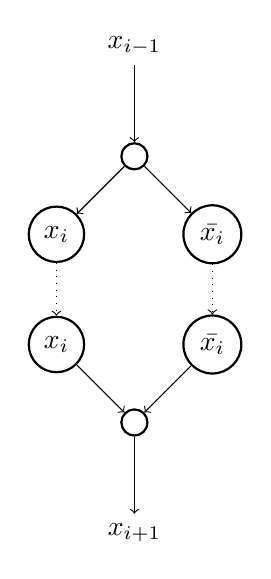
\begin{tikzpicture}[node distance={14mm}, main/.style = {draw, thick, circle}]
			\node (x-1) {$x_{i - 1}$};
			\node[main, below of = x-1] (e) {};
			\node[main, below left of = e] (x) {$x_i$};
			\node[main, below right of = e] (notx) {$\bar{x_i}$};
			\node[main, below of = x] (phx) {$x_i$};
			\node[main, below of = notx] (phnotx) {$\bar{x_i}$};
			\node[main, below right of = phx] (end) {};
			\node[below of = end] (x+1) {$x_{i + 1}$};
			\draw[->] (x-1) edge (e);
			\draw[->] (end) edge (x+1);
			\draw[->] (e) edge (x);
			\draw[->] (e) edge (notx);
			\draw[->, dotted] (x) edge (phx);
			\draw[->, dotted] (notx) edge (phnotx);
			\draw[->] (phx) edge (end);
			\draw[->] (phnotx) edge (end);
		\end{tikzpicture}
		\caption{Gadget for variables $x_i$.}
		\label{variable gadget}
	\end{subfigure}
	\begin{subfigure}{0.68\textwidth}\centering
		\begin{tikzpicture}[node distance={13mm}, main/.style = {draw, thick, circle}]
			\node[main] (startx0) {};
			\node[below of = startx0] (labelx0) {$x_0$};
			\node[main, below left of = startx0] (x0) {};
			\node[main, below right of = startx0] (notx0) {};
			\node[main, below of = x0] (phx0) {};
			\node[main, below of = notx0] (phnotx0) {};
			\node[main, below right of = phx0] (endx0) {};
			
			\node[below of = endx0] (gap) {};
			
			\node[main, below of = gap] (startxk) {};
			\node[below of = startxk] (labelxk) {$x_k$};
			\node[main, below left of = startxk] (xk) {};
			\node[main, below right of = startxk] (notxk) {};
			\node[main, below of = xk] (phxk) {};
			\node[main, below of = notxk] (phnotxk) {};
			\node[main, below right of = phxk] (endxk) {};
			
			\node[left of = endxk] (phantom0) {};
			\node[left of = phantom0] (phantom1) {};
			\node[left of = phantom1] (phantom2) {};
			\node[main, left of = phantom2] (c0) {$c_0$};
			\node[main, above of = c0] (c1) {$c_1$};
			\node[main, above of = c1] (c2) {$c_2$};
			\node[above of = c2] (gapc) {};
			\node[main, above of = gapc] (cl) {$c_l$};
			
			\draw[->] (startx0) edge (x0);
			\draw[->] (startx0) edge (notx0);
			\draw[->] (x0) edge (phx0);
			\draw[->] (notx0) edge (phnotx0);
			\draw[->] (phx0) edge (endx0);
			\draw[->] (phnotx0) edge (endx0);
			
			\draw[->, dotted] (endx0) edge (startxk);
			
			\draw[->] (startxk) edge (xk);
			\draw[->] (startxk) edge (notxk);
			\draw[->] (xk) edge (phxk);
			\draw[->] (notxk) edge (phnotxk);
			\draw[->] (phxk) edge (endxk);
			\draw[->] (phnotxk) edge (endxk);
			
			\draw[->, bend left = 60] (endxk) edge (c0);
			\draw[->] (c0) edge (c1);
			\draw[->, bend right = 50] (c0) edge (c1);
			\draw[->, bend left = 50] (c0) edge (c1);
			\draw[->] (c1) edge (c2);
			\draw[->, bend right = 50] (c1) edge (c2);
			\draw[->, bend left = 50] (c1) edge (c2);
			\draw[->, dotted] (c2) edge (cl);
		\end{tikzpicture}
		\caption{Scheme of variables and clauses.}
		\label{clause var scheme}
	\end{subfigure}
	\caption{Gadgets for variables and for clauses.}
\end{figure}

And then for every clause we will have one vertex and every two consequent clauses will be connected by 3 edges. These will represent the given literals. Also the last variable will be connected to the first clause. The scheme can be seen on the picture \ref{clause var scheme}. Now we only need to connect these gadgets together.

For that we will introduce \textbf{switch} gadget which connects the two previously mentioned gadgets. The exact construction of the switch is shown on the picture \ref{switch}. But it is enough to see the scheme of the switch on the picture \ref{scheme analyse}.

\begin{figure}[!ht]\centering
	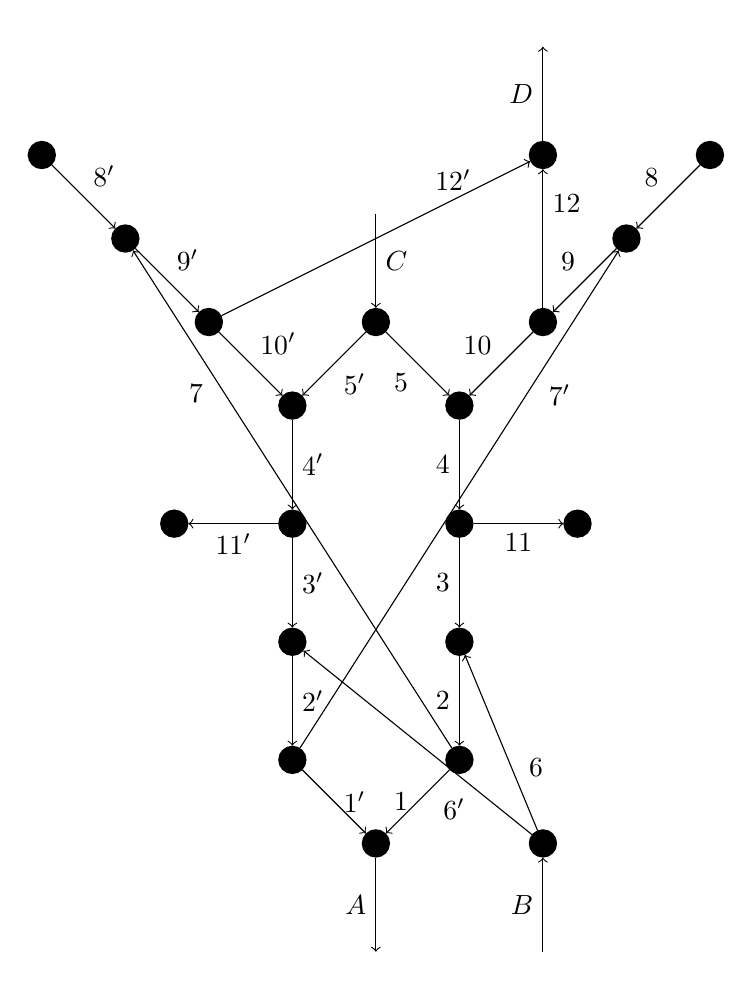
\begin{tikzpicture}[node distance={15mm}, main/.style = {draw, thick, circle, fill}]
		%% NODES
		% Start
		\node (1) {}; % Invisible start.
		\node[main, below of = 1] (2) {};
		% Left path
		\node[main, below left of = 2] (3) {};
		\node[main, below of = 3] (4) {};
		\node[main, below of = 4] (5) {};
		\node[main, below of = 5] (6) {};
		% Right path
		\node[main, below right of = 2] (3') {};
		\node[main, below of = 3'] (4') {};
		\node[main, below of = 4'] (5') {};
		\node[main, below of = 5'] (6') {};
		% End
		\node[main, below right of = 6] (7) {};
		\node[below of = 7] (8) {}; % Invisible end
		% Left wing		
		\node[main, above left of = 3] (9) {};
		\node[main, above left of = 9] (10) {};
		\node[main, above left of = 10] (11) {};
		% Right wing
		\node[main, above right of = 3'] (9') {};
		\node[main, above right of = 9'] (10') {};
		\node[main, above right of = 10'] (11') {};
		% Left arm
		\node[main, left of = 4] (12) {};
		% Right arm
		\node[main, right of = 4'] (12') {};
		% Rest of the graph.
		\node[main, above left of = 10'] (upper) {};
		\node[above of = upper] (ph-upper) {}; % Invisible upper
		\node[main, below right of = 6'] (lower) {};
		\node[below of = lower] (ph-lower) {}; % Invisible lower
		%% --S
		% Main two paths.
		\draw[->] (1) -- (2) node[midway, right] {$C$};
		\draw[->] (7) -- (8) node[midway, left] {$A$};
		\draw[->] (2) -- (3) node[midway, below right] {$5'$};
		\draw[->] (3) -- (4) node[midway, right] {$4'$};
		\draw[->] (4) -- (5) node[midway, right] {$3'$};
		\draw[->] (5) -- (6) node[midway, right] {$2'$};
		\draw[->] (6) -- (7) node[midway, right] {$1'$};
		\draw[->] (2) -- (3') node[midway, below left] {$5$};
		\draw[->] (3') -- (4') node[midway, left] {$4$};
		\draw[->] (4') -- (5') node[midway, left] {$3$};
		\draw[->] (5') -- (6') node[midway, left] {$2$};
		\draw[->] (6') -- (7) node[midway, left] {$1$};
		% Wings.
		\draw[->] (11) -- (10) node[midway, above right] {$8'$};
		\draw[->] (10) -- (9) node[midway, above right] {$9'$};
		\draw[->] (9) -- (3) node[midway, above right] {$10'$};
		\draw[->] (11') -- (10') node[midway, above left] {$8$};
		\draw[->] (10') -- (9') node[midway, above left] {$9$};
		\draw[->] (9') -- (3') node[midway, above left] {$10$};
		% Arms
		\draw[->] (4) -- (12) node[midway, below] {$11'$};
		\draw[->] (4') -- (12') node[midway, below] {$11$};
		% Rest of the graph.
		\draw[->] (ph-lower) -- (lower) node[midway, left] {$B$};
		\draw[->] (lower) -- (5) node[near start, below left]{$6'$};
		\draw[->] (lower) -- (5') node[near start, above right] {$6$};
		\draw[->] (upper) -- (ph-upper) node[midway, left] {$D$};
		\draw[->] (9) -- (upper) node[near end, above] {$12'$};
		\draw[->] (9') -- (upper) node[near end, right] {$12$};
		% The remaining two --s.
		\draw[->] (6) -- (10') node[near end, below right] {$7'$};
		\draw[->] (6') -- (10) node[near end, below left] {$7$};
	\end{tikzpicture}
	\caption{Switch construction.}
	\label{switch}
\end{figure}

\begin{figure}[!ht]\centering
	\begin{subfigure}{0.45\textwidth}\centering
		\begin{tikzpicture}[node distance={10mm}, main/.style = {draw, thick, circle}]
			\node[main] (O1) {};
			\node[main, right of = O1] (O2) {};
			\node[main, right of = O2] (O3) {};
			\node[main, right of = O3] (O4) {};
			\node[main, right of = O4] (O5) {};
			\node[main, right of = O5] (O6) {};
			\node[main, below of = O1] (O7) {};
			\node[main, right of = O7] (O8) {};
			\node[main, right of = O8] (O9) {};
			\node[main, right of = O9] (O10) {};
			\node[main, right of = O10] (O11) {};
			\node[main, right of = O11] (O12) {};
			
			\node[above of = O2] (8) {$8$};
			\node[above of = O3, color = myorange] (C) {$C$};
			\node[above of = O4, color = myblue] (D) {$D$};
			\node[above of = O5] (8') {$8'$};
			\node[below of = O8] (11) {$11$};
			\node[below of = O9, color = myorange] (A) {$A$};
			\node[below of = O10, color = myblue] (B) {$B$};
			\node[below of = O11] (11') {$11'$};
			
			\path[thick] (O1) edge (O2)
				(O2) edge (O3)
				(O3) edge (O4)
				(O4) edge (O5)
				(O5) edge (O6)
				(O7) edge (O8)
				(O7) edge (O1)
				(O8) edge (O9)
				(O9) edge (O10)
				(O10) edge (O11)
				(O11) edge (O12)
				(O12) edge (O6);
			\draw[->] (8) edge (O2);
			\draw[->, color = myorange] (C) edge (O3);
			\draw[->, color = myblue] (O4) edge (D);
			\draw[->] (8') edge (O5);
			\draw[->] (O8) edge (11);
			\draw[->, color = myorange] (O9) edge (A);
			\draw[->, color = myblue] (B) edge (O10);
			\draw[->] (O11) edge (11');
		\end{tikzpicture}
		\caption{Scheme for analyzing.}
		\label{scheme analyse}
	\end{subfigure}
	\begin{subfigure}{0.45\textwidth}\centering
		\begin{tikzpicture}[node distance={20mm}, main/.style = {draw, thick, circle}]
			\node[main] (8) {$8$};
			\node[main, fill, above of = 8] (phantom) {};
			\node[main, above of = phantom] (11) {$11$};
			\node[main, dashed, right of = phantom] (mid) {};
			\node[main, fill, right of = mid] (phantom') {};
			\node[main, below of = phantom'] (8') {$8'$};
			\node[main, above of = phantom'] (11') {$11'$};
			\node[above right of = mid, color = myred] (D) {$D$};
			\node[above left of = mid, color = myblue] (C) {$C$};
			\node[below right of = mid, color = myred] (B) {$B$};
			\node[below left of = mid, color = myblue] (A) {$A$};
			
			\draw[->] (8) edge (11);
			\draw[->] (8') edge (11');
			\draw[dashed] (phantom) edge (phantom');
			\draw[->, bend right = 20, color = myblue] (mid) edge (A);
			\draw[->, bend left = 20, color = myred] (B) edge (mid);
			\draw[->, bend left = 20, color = myblue] (C) edge (mid);
			\draw[->, bend right = 20, color = myred] (mid) edge (D);
		\end{tikzpicture}
		\caption{Drawn switch scheme.}
	\end{subfigure}
	\caption{Switch scheme.}
	\label{switch scheme}
\end{figure}


We may see that the switch is a small graph with 4 "inputs" $B, C, 8, 8'$ and 4 "outputs" $A, D, 11, 11'$. It can be shown that this graph has two following properties.

\begin{enumerate}
	\item If there are 2 edge disjoint paths one leaving at \textcolor{myorange}{$A$} and the other entering at \textcolor{myblue}{$B$}, then the former is entering at \textcolor{myorange}{$C$} and the later leaving at \textcolor{myblue}{$D$}. Look at the picture \ref{scheme analyse}.
	\item And exactly one more edge-disjoint path through the graph exists and it is either $8 \to 11$ or $8' \to 11'$.
\end{enumerate}

These switches can be connected by combining $A$ and $C$ and also $B$ and $D$. Therefore we insert the switches so $8 \to 11$ is for the variable in the clause gadget and the other ($8' \to 11'$) is replaced for the variable in the variable clause. After that we arbitrarily connect all switches together. Lastly we also insert vertices \textcolor{myviolet}{$W, X, Y, Z$} as shown on the global picture \ref{global scheme}.

\begin{figure}[!ht]\centering
		\begin{tikzpicture}[node distance={15mm}, main/.style = {draw, thick, circle}]
		\node[main] (startx0) {};
		\node[below of = startx0] (labelx0) {$x_0$};
		\node[main, below left of = startx0] (x0) {};
		\node[main, below right of = startx0] (notx0) {};
		\node[main, fill, below of = notx0] (dotx0) {};
		\node[below of = x0] (invdotx0) {};
		\node[main, below of = dotx0] (phnotx0) {};
		\node[main, below of = invdotx0] (phx0) {};
		\node[main, below right of = phx0] (endx0) {};
		
		\node[below of = endx0] (gap) {};
		
		\node[main, below of = gap] (startxk) {};
		\node[below of = startxk] (labelxk) {$x_k$};
		\node[main, below left of = startxk] (xk) {};
		\node[main, below right of = startxk] (notxk) {};
		\node[main, fill, below of = xk] (dotxk) {};
		\node[below of = notxk] (invdotxk) {};
		\node[main, below of = dotxk] (phxk) {};
		\node[main, below of = invdotxk] (phnotxk) {};
		\node[main, below right of = phxk] (endxk) {};
		
		\node[left of = endxk] (phantom0) {};
		\node[left of = phantom0] (phantom1) {};
		\node[left of = phantom1] (phantom2) {};
		\node[main, left of = phantom2] (c0) {$c_0$};
		\node[main, fill, above right of = c0] (dotc0) {};
		\node[main, above left of = dotc0] (c1) {$c_1$};
		\node[main, fill, above of = c1] (dotc1) {};
		\node[main, above of = dotc1] (c2) {$c_2$};
		\node[above of = c2] (gapc) {};
		\node[above of = gapc] (gapcc) {};
		\node[main, above of = gapcc] (cl) {$c_l$};
		
		\draw[->] (startx0) edge (x0);
		\draw[->] (startx0) edge (notx0);
		\draw[->] (x0) edge (phx0);
		\draw[->] (notx0) edge (phnotx0);
		\draw[->] (phx0) edge (endx0);
		\draw[->] (phnotx0) edge (endx0);
		
		\draw[->, dotted] (endx0) edge (startxk);
		
		\draw[->] (startxk) edge (xk);
		\draw[->] (startxk) edge (notxk);
		\draw[->] (xk) edge (phxk);
		\draw[->] (notxk) edge (phnotxk);
		\draw[->] (phxk) edge (endxk);
		\draw[->] (phnotxk) edge (endxk);
		
		\draw[->, bend left = 60] (endxk) edge (c0);
		\draw[->] (c0) edge (c1);
		\draw[bend right = 30] (c0) edge (dotc0);
		\draw[->, bend right = 30] (dotc0) edge (c1);
		\draw[->, bend left = 50] (c0) edge (c1);
		\draw[->] (c1) edge (c2);
		\draw[->, bend right = 50] (c1) edge (c2);
		\draw[->, bend left = 50] (c1) edge (c2);
		\draw[->, dotted] (c2) edge (cl);
		
		\draw[dashed] (dotc0) -- (dotxk) node[main, midway] (mid0) {};
		\draw[dashed] (dotc1) -- (dotx0) node[main, midway] (mid1) {};
		
		\node[above left of = mid0, color = myblue] (C0) {$C$};
		\node[above of = mid0, color = myred] (D0) {$D$};
		\node[below right of = mid0, color = myred] (B0) {$B$};
		\node[below of = mid0, color = myblue] (A0) {$A$};
		
		\node[above left of = mid1, color = myblue] (C1) {$C$};
		\node[above of = mid1, color = myred] (D1) {$D$};
		\node[below right of = mid1, color = myred] (B1) {$B$};
		\node[below of = mid1, color = myblue] (A1) {$A$};
		
		\draw[->, bend left = 20, color = myblue] (C0) edge (mid0);
		\draw[->, bend left = 20, color = myred] (B0) edge (mid0);
		\draw[->, bend right = 20, color = myblue] (mid0) edge (A0);
		\draw[->, bend right = 20, color = myred] (mid0) edge (D0);
		
		\draw[->, bend left = 20, color = myblue] (C1) edge (mid1);
		\draw[->, bend left = 20, color = myred] (B1) edge (mid1);
		\draw[->, bend right = 20, color = myblue] (mid1) edge (A1);
		\draw[->, bend right = 20, color = myred] (mid1) edge (D1);
		
		\draw[->, dashed, bend right = 20, color = myred] (D0) edge (B1);
		\draw[->, dashed, bend right = 20, color = myblue] (A1) edge (C0);
		
		\node[below of = A0, color = myviolet] (X) {$X$};
		\node[below of = B0, color = myviolet] (Y) {$Y$};
		\node[above of = cl, color = myviolet] (Z) {$Z$};
		\node[above of = C1, color = myviolet] (W) {$W$};
		
		\draw[->] (A0) edge (X);
		\draw[->] (Y) edge (B0);
		\draw[->] (W) edge (C1);
		\draw[->] (cl) edge (Z);
		\draw[->, bend left = 70] (D1) edge (startx0);
	\end{tikzpicture}
	\caption{Global scheme of the 3-SAT.}
	\label{global scheme}
\end{figure}

\begin{claim}
	$F$ is satisfiable $\Leftrightarrow$ there are edge disjoint paths from $W$ to $X$ and from $Y$ to $Z$.
\end{claim}

That can be seen on the global scheme. Important note is that for example if $x_i$ is set to true then the variable gadget uses $\bar{x_i}$ in the subgraph of $G$. Generally it uses the other path so it enforces the correct values in the clauses and also the other way around.
